\subsection{Codage compact des haplotypes humains}\label{sec:cohortecompacte}
La même fenêtre du chromosome 21 est reconstruite sur les deux haplotypes de 512 individus de phase 3 du projet 1000 Genomes~\cite{thousandgenomes}. Elle couvre les positions 20\,000\,001 à 20\,032\,768 de GRCh37. Le filtre retient 912 SNP et 38 autres variants courts bialléliques dont tous les génotypes sélectionnés sont phasés. Les 1\,024 séquences comptent de 32\,736 à 32\,775 bases.

Pour le score unitaire, le front \(F_e(k)\) atteint le plus grand indice \(i\) accessible avec \(e\) éditions sur la diagonale \(k=i-j\), après prolongement des identités. Le front inverse \(R_{e'}\) mesure la distance parcourue depuis la fin. Si \(n=|A|\) et \(m=|B|\), les fronts se rejoignent dès que
\[
  F_e(k)+R_{e'}(n-m-k)\geq n,\qquad
  d=\min(e+e').
\]
Les deux sens progressent à tour de rôle~\cite{wfa,biwfa}. Le premier mot de huit bases compare les octets. Les extensions suivantes lisent, au choix, huit bases en octets ou 32 bases en deux bits par mot de 64 bits. Une lettre hors de \(\{A,C,G,T\}\), une demande de CIGAR ou un score supérieur à 96 déclenchent le repli vers BiWFA.

La figure~\ref{fig:cohortecompacte} compare les temps sur un nœud EPYC réservé. À charge fixe, \(E_p=T_1/(pT_p)\). Pour le plan faible, \(E_p=(P_p/P_1)T_1/(pT_p)\), où \(P_p\) désigne le nombre de paires. Le quotient \(P_p/p\) varie de 8\,128 à 8\,184 par cœur selon l’arrondi du nombre d’haplotypes.

\begin{figure}[htbp]
\centering
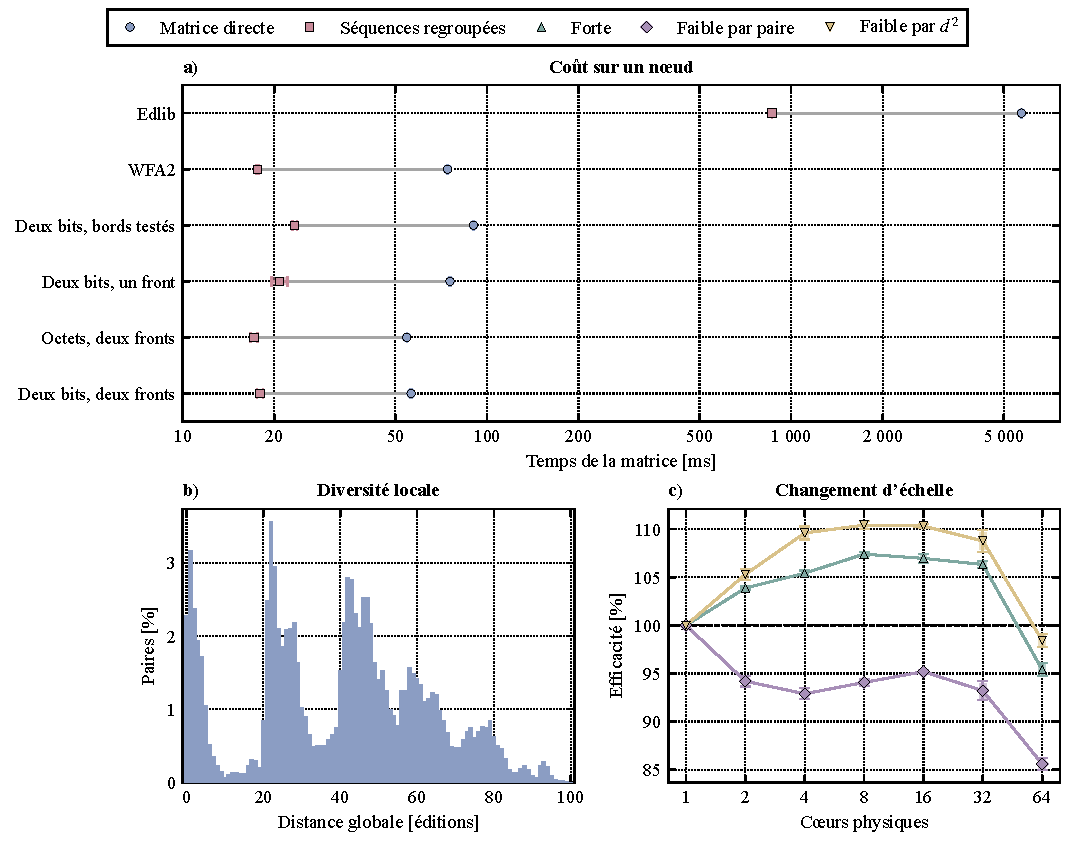
\includegraphics[width=.93\linewidth]{../figures/cpu/cohorte_compacte.pdf}
\caption{Le temps de matrice comprend la préparation et la restitution des scores. La distribution porte sur toutes les paires. Les marques donnent les moyennes de cinq blocs après échauffement, les traits épais leur écart-type et les traits fins l’intervalle à 95\,\%. Pour l’efficacité, l’incertitude du rapport propage celle des deux temps.}\label{fig:cohortecompacte}
\sourcefig{python/studies/cohorte_compacte.py}
\end{figure}
\FloatBarrier
À codage fixé, les sentinelles réduisent le temps moyen de 16,3\,\%. Le parcours bidirectionnel réduit ensuite de 25,5\,\% le temps du front unique. Sur les 8\,128 paires du profil monocœur, le codage en deux bits ramène les défauts L1D de 1092,0 à 266,7 par paire. Les mots compactés occupent 8\,396\,968 octets en plus des séquences originales. La matrice directe prend 54,51~ms en octets et 56,31~ms en deux bits sur 64 cœurs.

La médiane vaut 42 éditions et 11\,954 paires ont la distance nulle. Les 386 séquences distinctes demandent 74\,305 alignements après regroupement. Les 523\,776 scores sont ensuite restitués dans l’ordre des haplotypes. Sur 64 cœurs, cette opération porte les temps totaux à 17,61~ms pour WFA2 et à 17,94~ms pour les deux bits. D’un à 64 cœurs, l’efficacité des fronts compactés atteint 95,4\,\% à matrice fixe et 85,6\,\% à nombre de paires par cœur comparable. La moyenne de \(d^2\) passe de 1\,852,50 à 2\,130,57 entre les deux préfixes. Pondérée par \(d^2\), indicateur du nombre d’états des fronts, l’efficacité faible vaut 98,4\,\%.

\synthese{À 64 cœurs, les fronts compactés calculent la matrice directe en 56,31 \(\pm\) 0,32~ms, contre 74,24 \(\pm\) 0,26~ms pour WFA2. Le rapport des temps moyens vaut 1,32 pour WFA2 et 101,45 pour Edlib.}
